\documentclass[../thesis/thesis.tex]{subfiles}
\begin{document}

\chapter{Evaluation}
\label{chap:evaluation}

We believe it is possible to produce a VC investment screening system that is efficient, robust and powerful. In the previous chapter, we describe the development and structure of such a system. Our system is based around identifying startup companies that are likely to receive additional funding or a liquidity event (exit) in a given forecast window. This system can generate statistics and make recommendations that may assist VC firms to efficiently and effectively screen investment candidates. In this chapter, we evaluate models developed by our system against criteria of efficiency, robustness and predictive power. We discuss our findings more broadly and their implications for investors and future research into startup investment and performance.

In the previous chapter, we produced a classification pipeline which we optimised with respect to the robustness of its performance over time. In this chapter, we evaluate the performance of models produced by this pipeline against a held-out test dataset. This evaluation process is depicted in \ref{fig:evaluation:pipeline_evaluation}. We use the pipeline to fit a model to a dataset sliced from the master database. We apply this model to another feature vector from the master database and make predictions. We score these predictions against truth values derived from the held-out test database (c. Apr-17). This process is performed multiple times to evaluate our three primary criteria derived from our literature review: efficiency, robustness and predictive power. In this chapter, we evaluate our system against that criteria.The experiments are as follows: efficiency, the pipeline is fitted to datasets of various sample sizes; robustness, the pipeline is fitted to datasets from various time slices; and predictive power, the forecast window between the feature vector and outcome is varied.

Firstly, we evaluate efficiency by exploring the learning curves of our classification techniques and whether there is sufficient data to produce reliable statistics. We also evaluate efficiency with respect to accuracy at different levels of feature abstraction (e.g. feature grouping based on our conceptual framework). Secondly, we evaluate robustness by evaluating our models against multiple reverse-engineered historical datasets and measuring their variance. Thirdly, we evaluate predictive power by testing different forecast windows outcomes and evaluating our models’ accuracy for startups at different stages of their development lifecycle.

\begin{figure}[!htb]
    \centering
    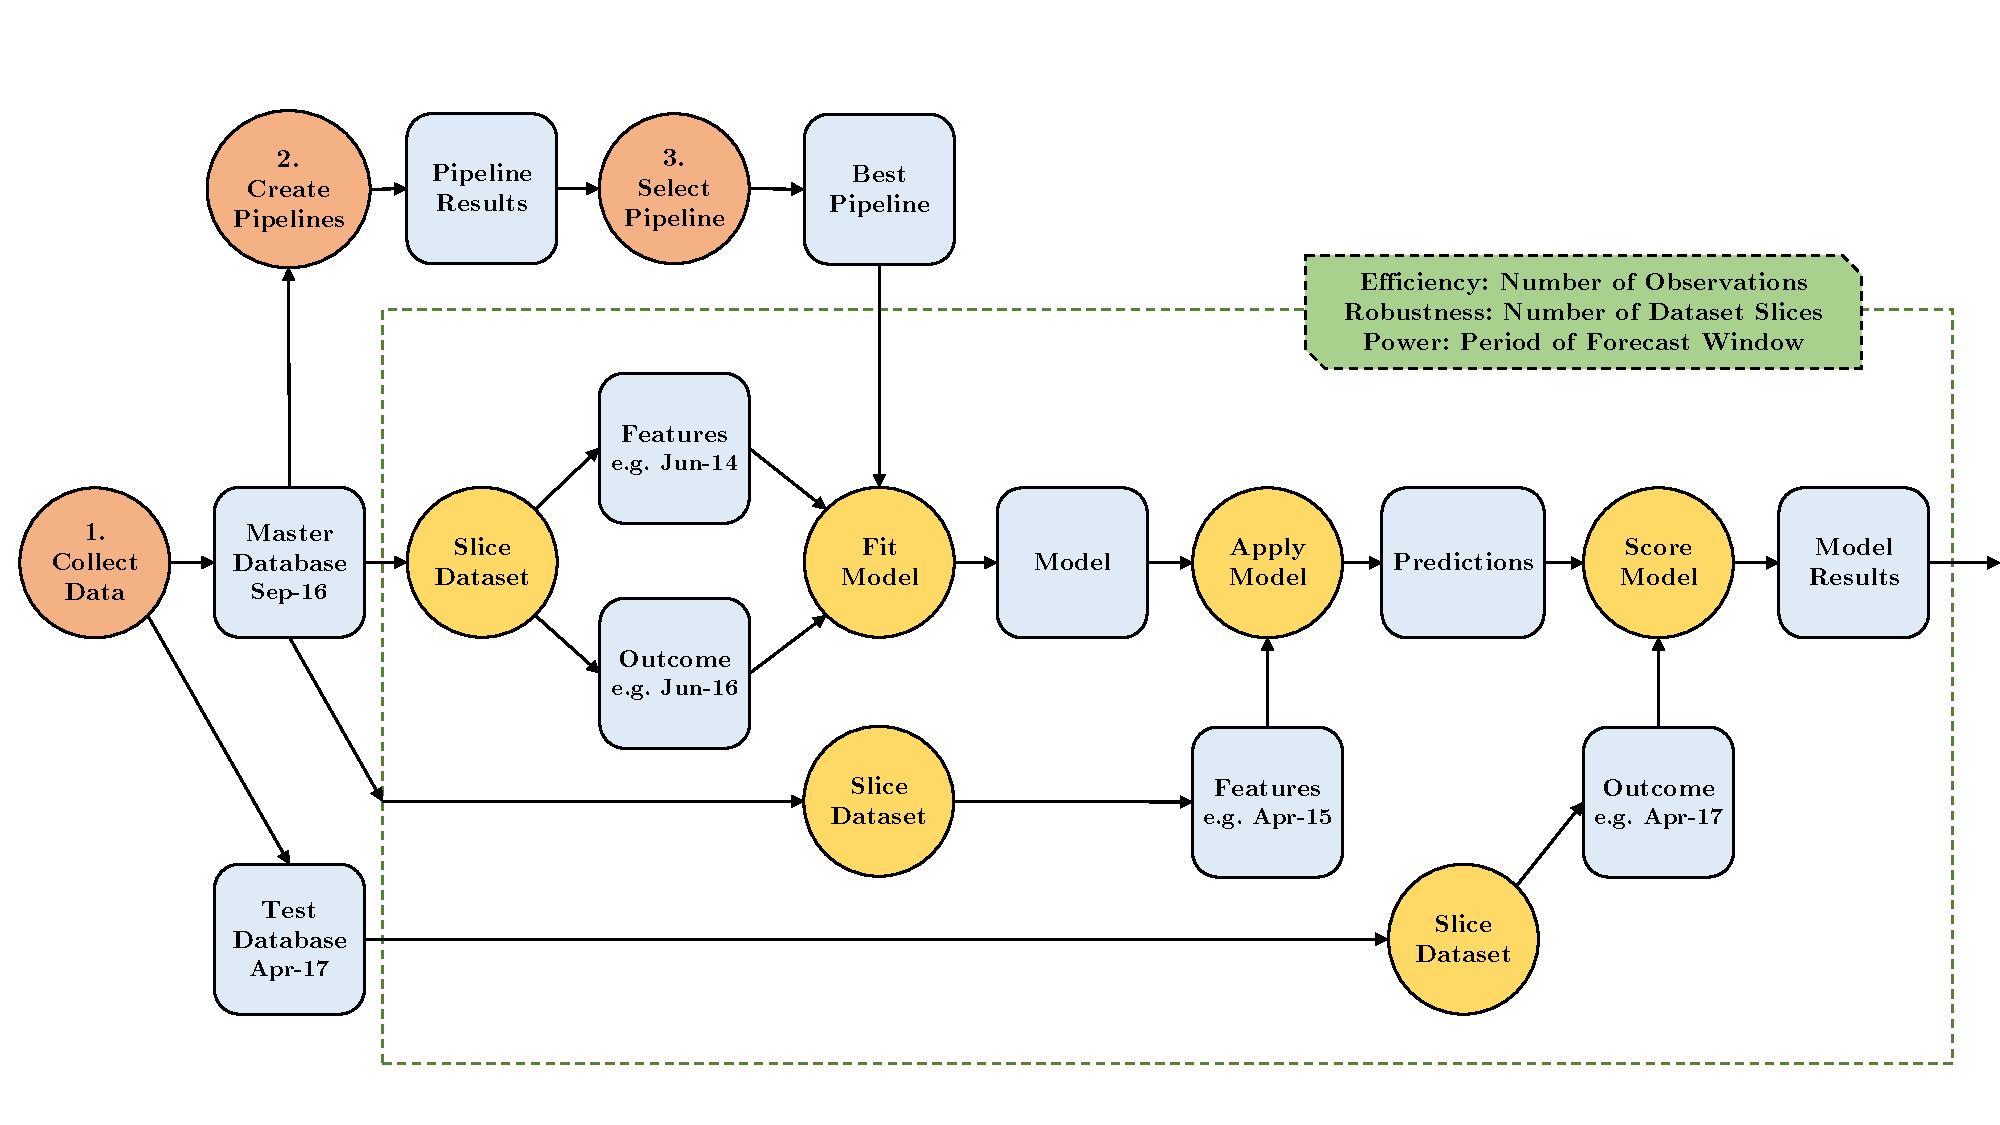
\includegraphics[width=\textwidth]{../figures/evaluation/pipeline_evaluation}
    \caption[Pipeline evaluation flowchart]{Pipeline evaluation overview.}
    \label{fig:evaluation:pipeline_evaluation}
\end{figure}

\section{Efficiency}

A rationale for this research project is the need for more efficient forms of \gls{vc} investment analysis which leverage technology, particularly in surfacing and screening. By its nature, our automated system should be more efficient than current manual methods but it's also important to determine how to most efficiently use the data that we have. %TODO - Write paragraph

\subsection{Dataset Size}

For these reasons, we decided to investigate the learning curves for our classification pipeline to determine whether we could use smaller samples from our dataset to achieve similar predictive power and reduce our need for computational power and time taken. We used cross-validation to split our dataset 10 times and used subsets of the training set with varying sizes to train the estimator and produce training and test scores for each subset size. The convergence or divergence of our training and cross-validation curves will imply whether our classification pipeline is over- or under-fitting our data for various sizes allowing us to select an optimal sample size. %TODO - Write paragraph

\begin{figure}[!htb]
    \centering
    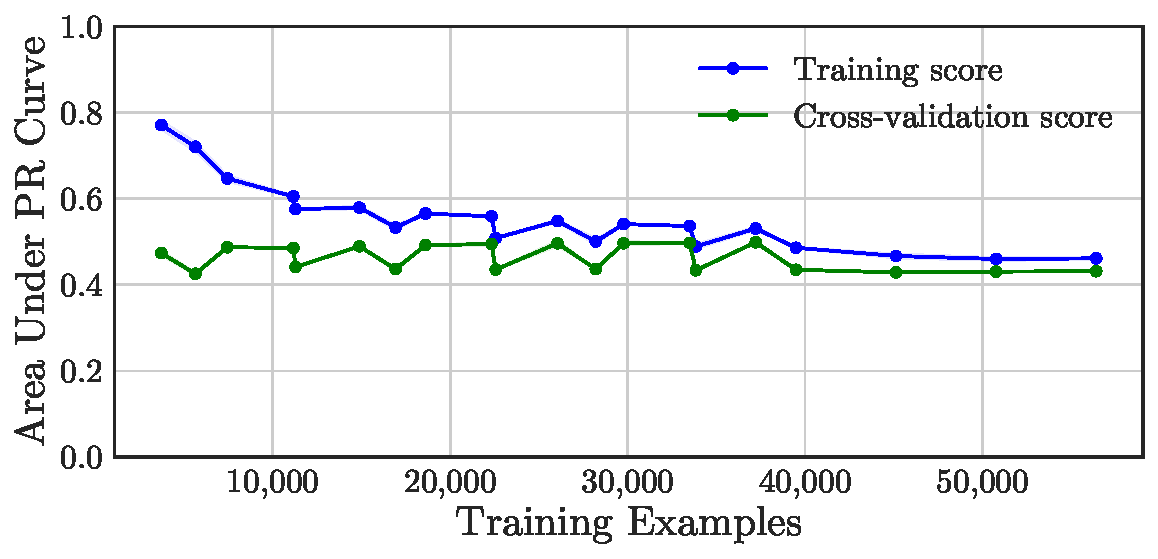
\includegraphics[width=\textwidth]{../figures/evaluation/efficiency_learning_curve} %TODO - Fix for different curves
    \caption[Learning curve]{}
    \label{fig:evaluation:efficiency_learning_curve}
\end{figure}

\subsection{Time Profile}

We will also investigate the time profiling of the system to determine whether the system is practical for use in the \gls{vc} industry. %TODO - Write paragraph

%Figure Time by training_observations - ???

\section{Robustness}

It is critical that our system be robust with respect to time so investors can rely on its predictions based on historical models. CrunchBase provides created and last-updated timestamps for each record in their CSV-formatted dumps (and also in the JSON-formatted responses from their API). We took advantage of this to produce a system that reverse-engineers previous database states by filtering the current database by only records that were created by a given 'slice' date.

We performed preliminary testing of this technique by comparing a historical CrunchBase database collected in December 2013 with a slice from our primary dataset collected in September 2016, as shown in Table~\ref{fig:evaluation:2013_slice_comparison}. While there are some differences in the records, particularly in the IPO relation, we consider this to be satisfactory variance considering the 3-year time period. The key relations for our purposes are Companies, Funding Rounds and People, all of which had minor differences considering the size of these datasets. Table~\ref{fig:evaluation:slice_counts_over_time} shows company counts by startup development stage from different dataset slices. We limited our experiments to dataset slices from 2012-onwards because prior to 2012 the datasets become too small to use to make predictions (particularly given the class imbalance).

\begin{figure}[!htb]
    \centering
    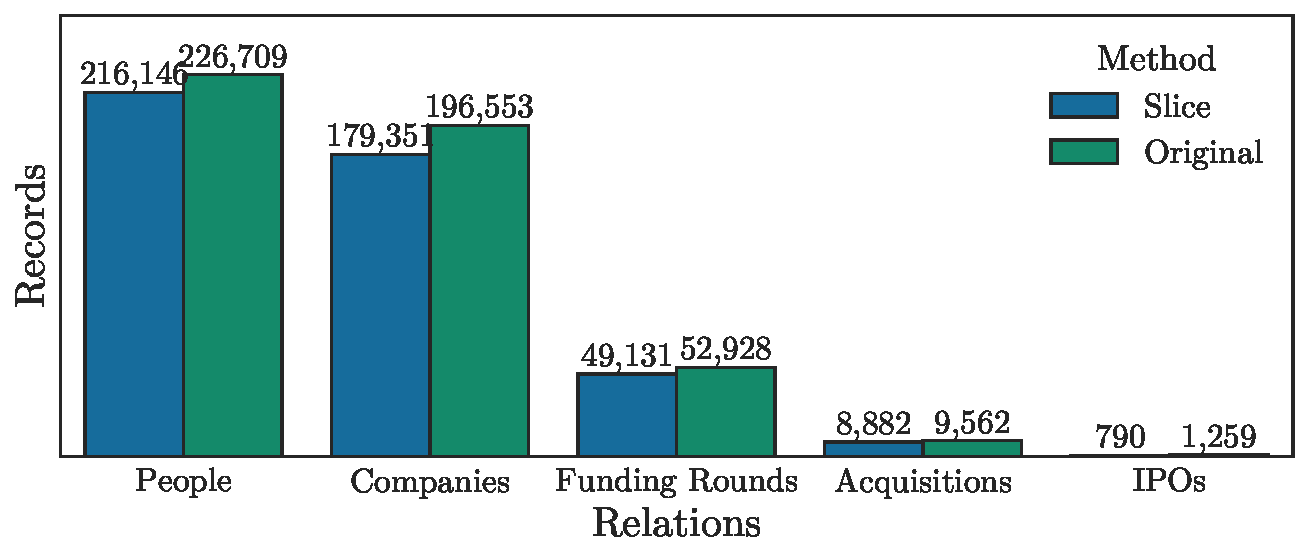
\includegraphics[width=\textwidth]{../figures/evaluation/2013_slice_comparison}
    \caption[Dataset slice compared with original dataset]{}
    \label{fig:evaluation:2013_slice_comparison}
\end{figure}

\begin{figure}[!htb]
    \centering
    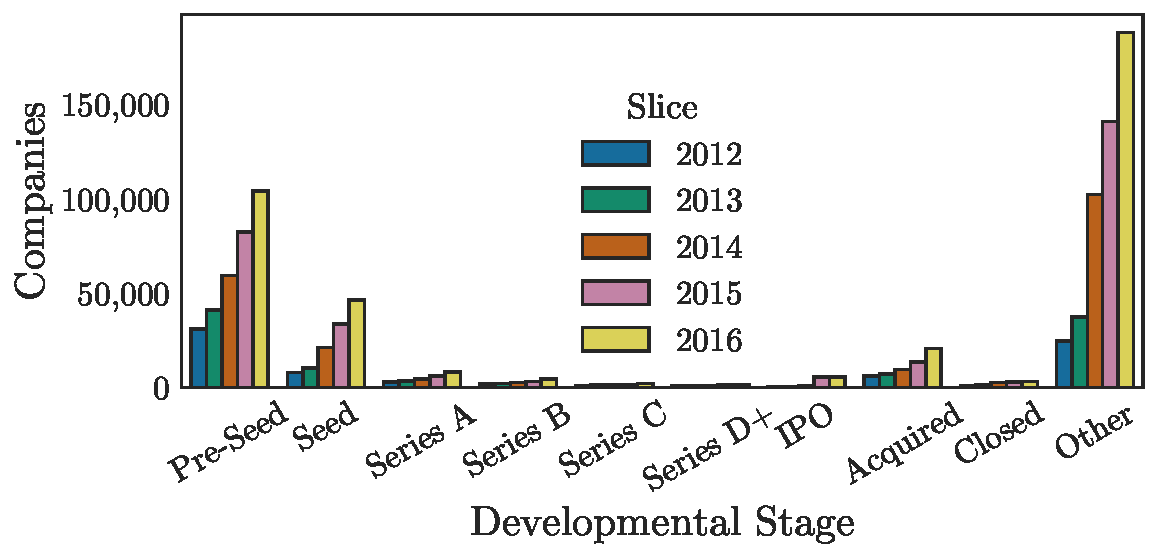
\includegraphics[width=\textwidth]{../figures/evaluation/slice_counts_over_time}
    \caption[Dataset counts over time]{}
    \label{fig:evaluation:slice_counts_over_time}
\end{figure}

%TODO

\begin{figure}[!htb]
    \centering
    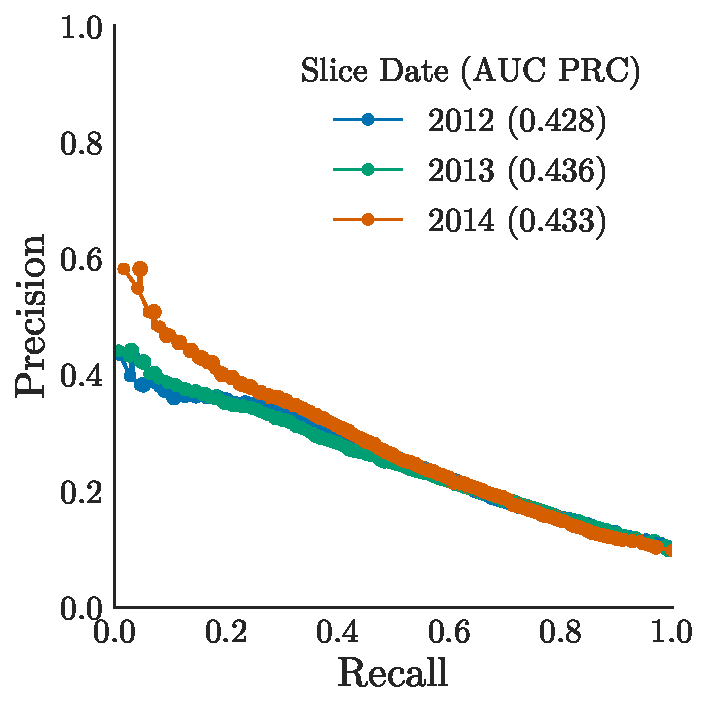
\includegraphics[width=\textwidth]{../figures/evaluation/pr_curve_slice}
    \caption[PR Curves by slice date]{}
    \label{fig:evaluation:pr_curve_slice}
\end{figure}

\begin{table}[!htb]
    \centering
    \scalebox{0.9}{\begin{tabular}{llrrrrrr} \toprule
\multicolumn{2}{l}{Slice Date} & N & (\%)    & Accuracy & Precision   & Recall & F1-Score \\ \midrule
2012 & Outcome=0 & 106,583 & (90.2\%) & - & 0.95 & 0.77 & 0.85 \\
     & Outcome=1 & 11,538 & (9.8\%) & - & 0.22 & 0.59 & 0.32 \\
     & Avg/Total & 118,121 & - & 0.76 & 0.88 & 0.76 & 0.80 \\
2013 & Outcome=0 & 106,489 & (90.2\%) & - & 0.95 & 0.75 & 0.84 \\
     & Outcome=1 & 11,535 & (9.8\%) & - & 0.21 & 0.62 & 0.32 \\
     & Avg/Total & 118,024 & - & 0.74 & 0.88 & 0.74 & 0.79 \\
2014 & Outcome=0 & 106,583 & (90.2\%) & - & 0.95 & 0.76 & 0.84 \\
     & Outcome=1 & 11,538 & (9.8\%) & - & 0.21 & 0.61 & 0.32 \\
     & Avg/Total & 118,121 & - & 0.74 & 0.88 & 0.74 & 0.79 \\
\bottomrule \end{tabular}
}
    \caption[Classification report by slice date]{}
    \label{fig:evaluation:clf_report_slice}
\end{table}


\begin{figure}[!htb]
    \centering
    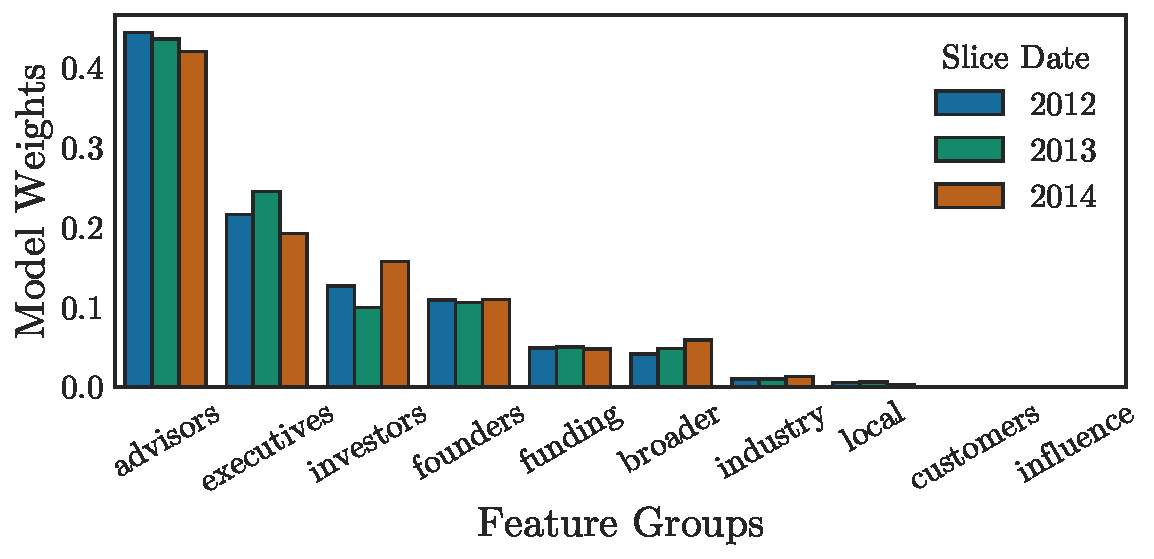
\includegraphics[width=\textwidth]{../figures/evaluation/feature_groups_slice}
    \caption[Grouped feature weights by slice date]{}
    \label{fig:evaluation:feature_groups_slice}
\end{figure}

\section{Predictive Power}

Finally, we test our system's predictive power for making forecasts of different time periods. We use the same system of reverse-engineering time slices that we used in our previous experiment to robustness, but this time we vary the time difference between the slice that provides our features and the slice that provides our label.

\subsection{Preliminary Analysis}

We performed preliminary testing by combining pair-wise datasets of each year from 2012-2016 inclusive and exploring the proportion of companies that raised additional funding or exited (for brevity, we will call this ``investment success''. Figure~\ref{fig:evaluation:outcome_forecast_window} shows how investment success varies with respect to the forecast window (time between the observed features and the measured outcome). Intuitively, we see a positive relationship between length of forecast window and investment success. In particular, very few companies appear to have investment success over a period of less than 2 years so we will focus our experimentation on forecast windows of 2--4 years.

\begin{figure}[!htb]
    \centering
    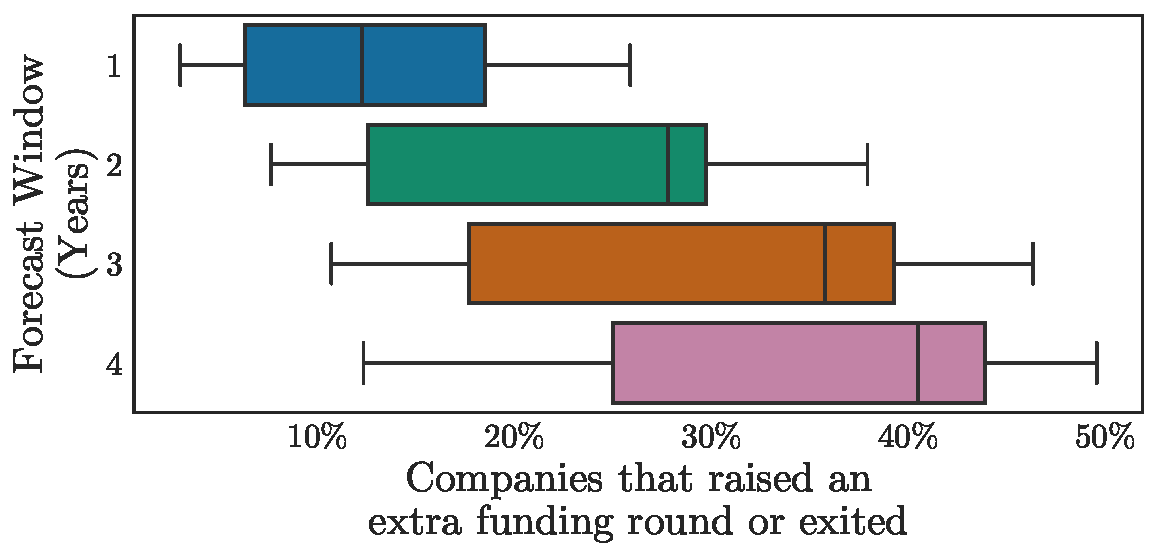
\includegraphics[width=\textwidth]{../figures/evaluation/outcome_forecast_window}
    \caption[Investment success by forecast window]{}
    \label{fig:evaluation:outcome_forecast_window}
\end{figure}

We also looked at how investment success varies with respect to development stage, shown in Figure~\ref{fig:evaluation:outcome_stage}. We see a broad positive relationship between developmental stage and likelihood of investment success, which we would expect as at each stage there is higher market traction and scrutiny from investors. One exception is for companies at Series D+ stage, but this may reflect that these companies are aiming for an exit which likely takes longer than seeking additional funding rounds and so is less well shown in our dataset (which caps out at a forecast window of 4 years). The variance between the different developmental stages suggests that in our experimentation we should investigate how our system predicts each stage independently, as well as in aggregate.

\begin{figure}[!htb]
    \centering
    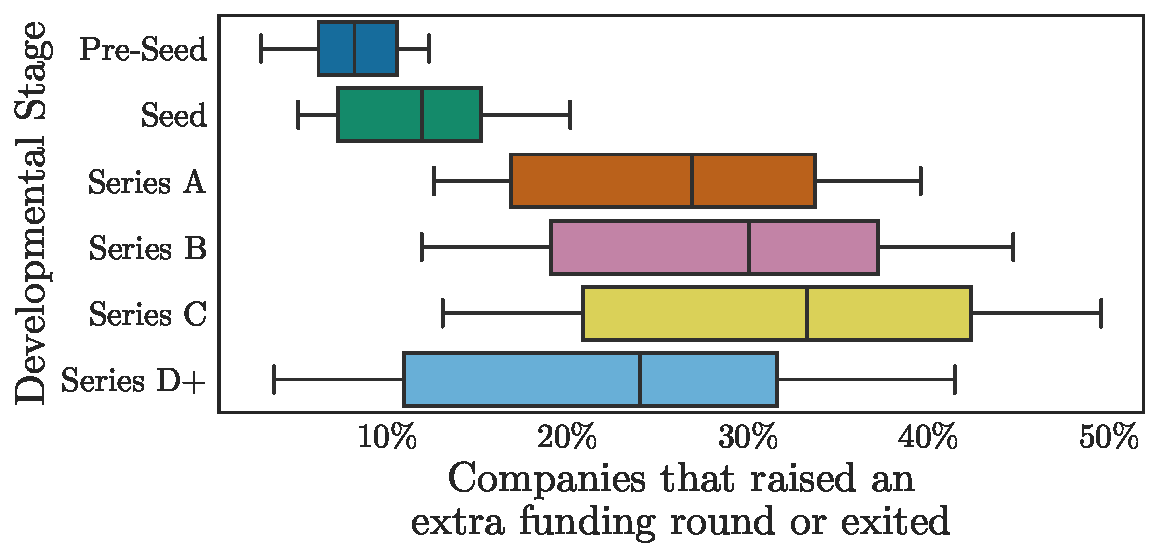
\includegraphics[width=\textwidth]{../figures/evaluation/outcome_stage}
    \caption[Investment success by developmental stage]{}
    \label{fig:evaluation:outcome_stage}
\end{figure}

\subsection{Forecast Windows}

\begin{figure}[!htb]
    \centering
    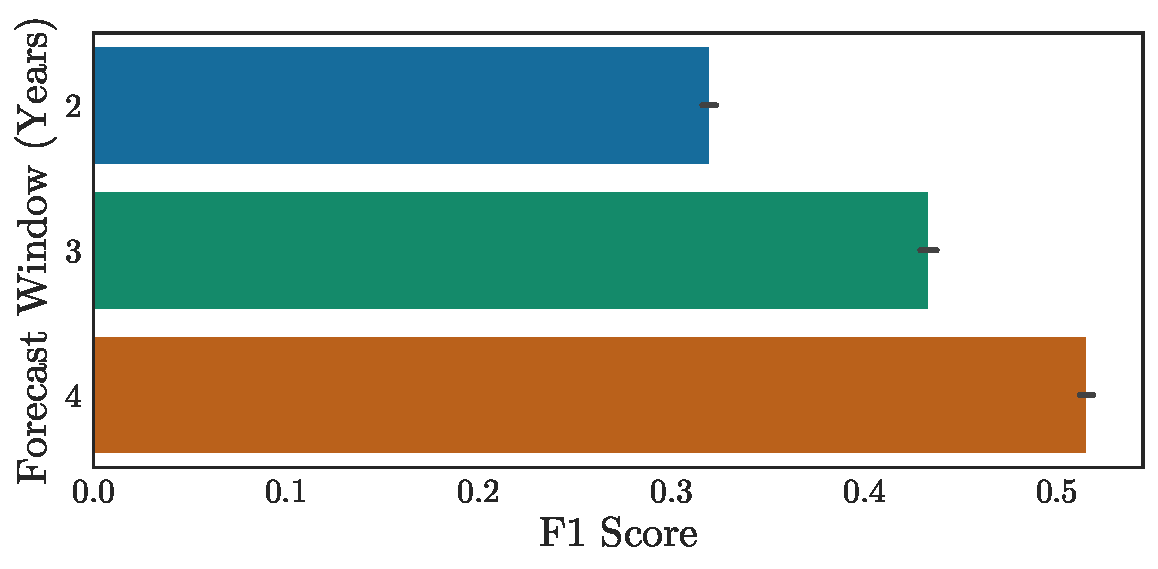
\includegraphics[width=\textwidth]{../figures/evaluation/predictive_window}
    \caption[F1 Scores by forecast window]{}
    \label{fig:evaluation:f1_predictive_window}
\end{figure}

\begin{table}[!htb]
    \centering
    \scalebox{0.9}{\begin{tabular}{llrrrrr} \toprule
Forecast Window  & & N (\%)    & Accuracy & Precision   & Recall & F1-Score \\ \midrule
2 Years & Outcome=0 & 319,655 (90.2\%) & - & 0.95 & 0.76 & 0.84 \\
        & Outcome=1 & 34,611 (9.8\%) & - & 0.22 & 0.61 & 0.32 \\
        & Avg/Total & 354,266 & 0.75 & 0.88 & 0.75 & 0.79 \\
3 Years & Outcome=0 & 216,816 (85.6\%) & - & 0.93 & 0.77 & 0.84 \\
        & Outcome=1 & 36,602 (14.4\%) & - & 0.32 & 0.66 & 0.43 \\
        & Avg/Total & 253,418 & 0.75 & 0.84 & 0.75 & 0.78 \\
4 Years & Outcome=0 & 137,217 (81.9\%) & - & 0.91 & 0.81 & 0.86 \\
        & Outcome=1 & 30,255 (19.1\%) & - & 0.43 & 0.65 & 0.52 \\
        & Avg/Total & 167,472 & 0.78 & 0.82 & 0.78 & 0.80 \\
\bottomrule \end{tabular}
}
    \caption[Classification report by forecast window]{}
    \label{fig:evaluation:clf_report_window}
\end{table}

\begin{figure}[!htb]
    \centering
    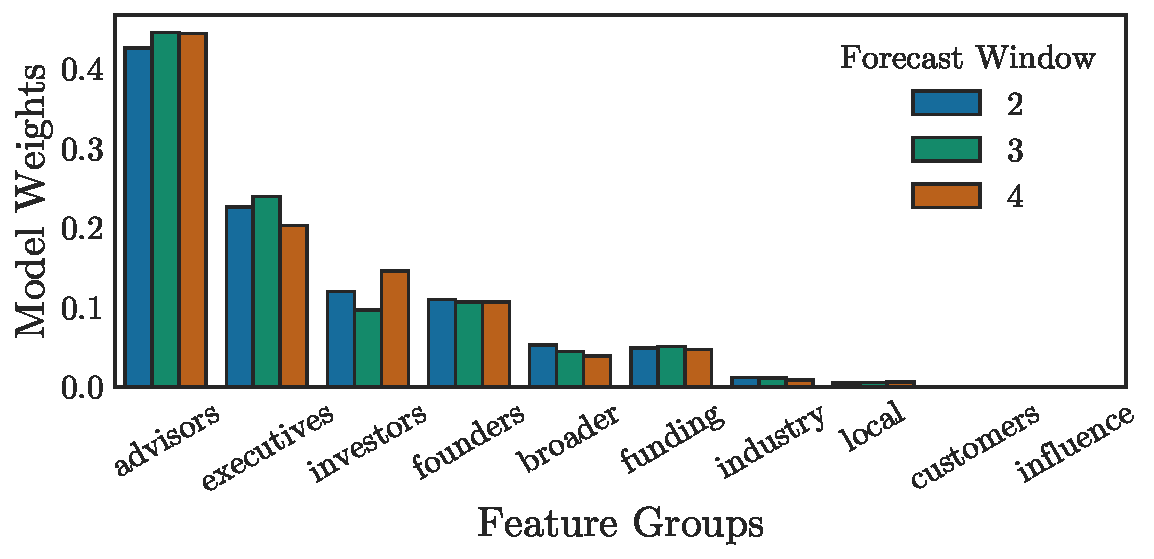
\includegraphics[width=\textwidth]{../figures/evaluation/feature_groups_window}
    \caption[Grouped feature weights by forecast window]{}
    \label{fig:evaluation:feature_groups_window}
\end{figure}

\subsection{Development Stage}

\begin{figure}[!htb]
    \centering
    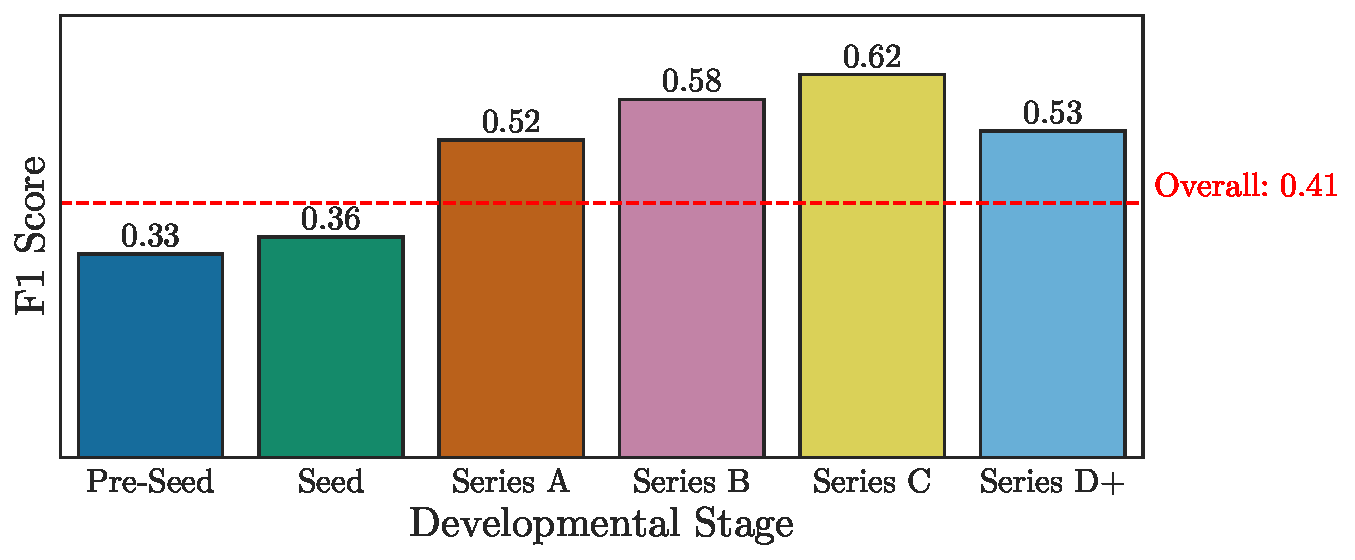
\includegraphics[width=\textwidth]{../figures/evaluation/predictive_stage}
    \caption[F1 Scores by developmental stage]{}
    \label{fig:evaluation:f1_predictive_stage}
\end{figure}

\begin{table}[!htb]
    \centering
    \scalebox{0.9}{\begin{tabular}{llrrrrrr} \toprule
\multicolumn{2}{l}{Stage} & N & (\%)    & Accuracy & Precision   & Recall & F1-Score \\ \midrule
Pre-Seed     & Outcome=0 & 491,154 & (90.4\%) & - & 0.94 & 0.88 & 0.91 \\
             & Outcome=1 & 51,862 & (9.6\%) & - & 0.27 & 0.42 & 0.33 \\
             & Avg/Total & 543,016 & - & 0.84 & 0.87 & 0.84 & 0.85 \\
Seed         & Outcome=0 & 136,586 & (85.7\%) & - & 0.93 & 0.60 & 0.73 \\
             & Outcome=1 & 22,872 & (14.3\%) & - & 0.24 & 0.74 & 0.36 \\
             & Avg/Total & 159,458 & - & 0.62 & 0.83 & 0.62 & 0.68 \\
Series A     & Outcome=0 & 23,861 & (67.6\%) & - & 0.87 & 0.18 & 0.30 \\
             & Outcome=1 & 11,427 & (32.4\%) & - & 0.36 & 0.94 & 0.52 \\
             & Avg/Total & 35,288 & - & 0.43 & 0.71 & 0.43 & 0.37 \\
Series B     & Outcome=0 & 12,116 & (59.3\%) & - & 0.84 & 0.04 & 0.07 \\
             & Outcome=1 & 8,314 & (40.7\%) & - & 0.41 & 0.99 & 0.58 \\
             & Avg/Total & 20,430 & - & 0.43 & 0.66 & 0.43 & 0.28 \\
Series C     & Outcome=0 & 5,555 & (55.2\%) & - & 0.82 & 0.03 & 0.07 \\
             & Outcome=1 & 4,516 & (44.8\%) & - & 0.45 & 0.99 & 0.62 \\
             & Avg/Total & 10,071 & - & 0.46 & 0.66 & 0.46 & 0.32 \\
Series D+    & Outcome=0 & 4,416 & (64.1\%) & - & 0.89 & 0.02 & 0.03 \\
             & Outcome=1 & 2,477 & (35.9\%) & - & 0.36 & 1.00 & 0.53 \\
             & Avg/Total & 6,893 & - & 0.37 & 0.70 & 0.37 & 0.21 \\
\bottomrule \end{tabular}
}
    \caption[Classification report by developmental stage]{}
    \label{fig:evaluation:clf_report_stage}
\end{table}

\begin{figure}[!htb]
    \centering
    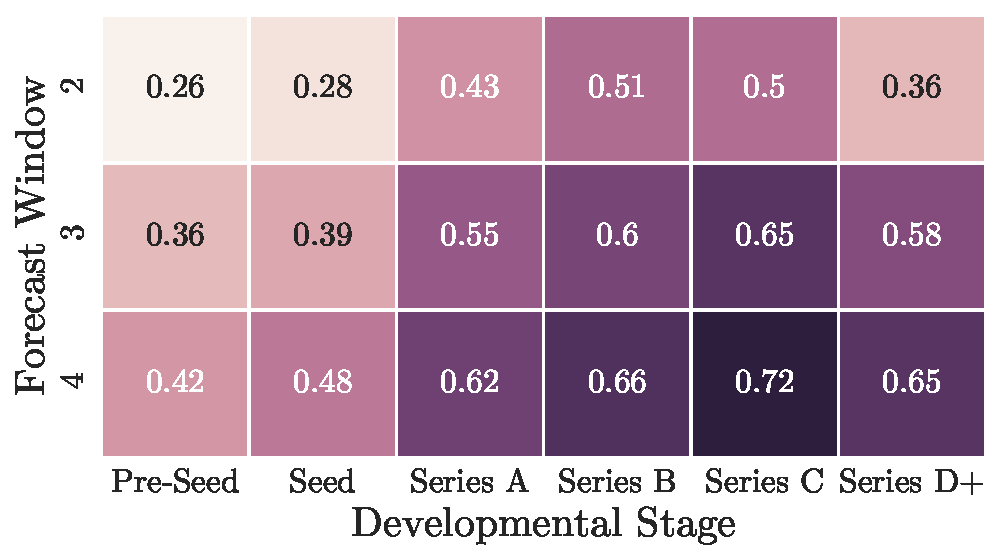
\includegraphics[width=\textwidth]{../figures/evaluation/predictive_heatmap}
    \caption[F1 Scores by developmental stage and forecast window]{}
    \label{fig:evaluation:f1_predictive_heatmap}
\end{figure}

\begin{figure}[!htb]
    \centering
    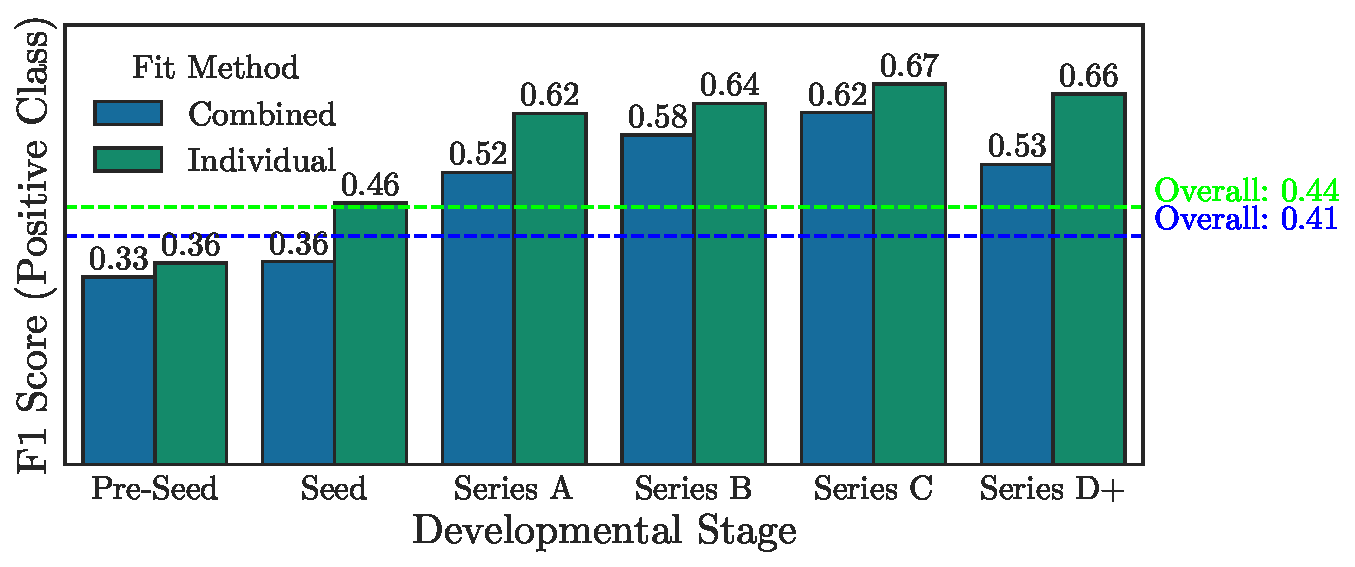
\includegraphics[width=\textwidth]{../figures/evaluation/f1_individual_overall}
    \caption[F1 Scores by moodel fit method]{}
    \label{fig:evaluation:f1_individual_overall}
\end{figure}

\begin{figure}[!htb]
    \centering
    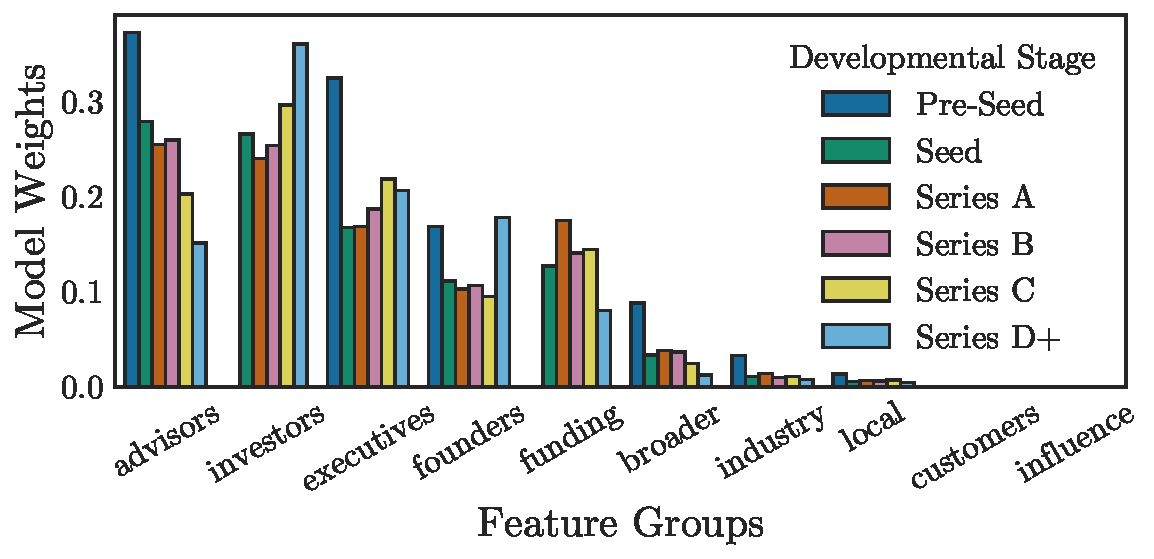
\includegraphics[width=\textwidth]{../figures/evaluation/feature_groups_stage}
    \caption[Grouped feature weights by developmental stage]{}
    \label{fig:evaluation:feature_groups_stage}
\end{figure}

\begin{table}[!htb]
    \centering
    \scalebox{0.9}{\begin{tabular}{lrrrrrrrrr} \toprule
& \multicolumn{3}{c}{Company} \\
Feature                 & Company1  & Company2  & Company3  \\ \midrule
Feature1                & Count1    & Count2    & Count3    \\
Feature2                & Count1    & Count2    & Count3    \\
Feature3                & Count1    & Count2    & Count3    \\ \midrule
P(Outcome=1 | X)        & Count1    & Count2    & Count3    \\
Predicted Outcome       & Count1    & Count2    & Count3    \\
Actual Outcome          & Count1    & Count2    & Count3    \\
Correct Prediction      & Count1    & Count2    & Count3    \\
\bottomrule \end{tabular}
} %TODO
    \caption[Three example company profiles and their predictions]{}
    \label{fig:evaluation:example_predictions}
\end{table}

\subsection{Target Outcomes}

% F1 by metric - Investment Successs vs. Exit vs. Additional Funding

% F1 - Exit by forecast window

% F1 - Exit by developmental stage

 \ifcsdef{mainfile}{}{\printbibliography}
\end{document}
